%\subsection{تخمین پارامترهای کانال رول موتور خاموش}
به منظور افزایش دقت تخمین پارامترها، در ابتدا پارامترهای مربوط به هر کانال جداگانه تخمین زده شده‌است و در ادامه پارامترهای مشترک کانال‌ها اصلاح شده‌اند.
%به علت زیاد بودن پارامترهای شبیه‌سازی چهارپره ابتدا پارامترهای هر کانال به‌صورت جداگانه (بدون در نظر گرفتن تاثیر متقابل دیگر کانال‌‌ها) اصلاح شدند. سپس، پارامترهای کانال رول-پیچ و در نهایت کانال رول-پیچ-یاو  (با در نظر گرفتن تاثیر متقابل دیگر کانال‌‌ها) اصلاح شدند.
 برای افزایش دقت، در کانال‌های رول و پیچ، ابتدا پارامترها به‌صورت موتور خاموش اصلاح شدند و سپس، پارامترهای مربوط به موتور اصلاح شدند.
در فرایند اصلاح پارامتر، بعد از هر مرحله اصلاح پارامتر اشاره‌شده در بالا،  پارامترهای اصلاح شده‌ی مرحله قبلی ثابت فرض شده‌اند و سایر پارامترها تخمین زده شده‌اند.
% به جعبه‌ابزار
% \lr{Parameter Estimator}
%داده شدند. 
برای اصلاح پارامتر هر مرحله چندین آزمایش با سناریوهای مختلف انجام شده‌است،
% و خروجی اصلاح پارامتر بر اساس تمام آزمایش‌های معتبر است
اما برای رعایت ایجاز از آوردن تمامی آزمایش‌ها پرهیز شده‌است.
% و تنها خروجی یک آزمایش آورده شده‌است.


%برای اصلاح پارامترها چندین آزمایش انجام شد و با استفاده از داده‌های ثبت شده از وضعیت استند و جعبه‌ابزار
%\lr{Parameter Estimator}، پارامترها اصلاح شدند.

برای انجام آزمایش، استند از شرایط اولیه مختلف و با ورودی‌های مختلف رها شده و از خروجی سنسور داده برداری شده‌است. سپس، مدل و داده‌های ثبت شده‌ی سنسور (وضعیت استند) به جعبه‌ابزار
\lr{Parameter Estimator} داده‌شده‌اند. 
وضعیت استند در شبیه‌سازی و واقعیت بعد از اصلاح پارامترهای مختلف
%\ref{roll_ml_ps1}, \ref{roll_ml_ps1}, \ref{roll_ml_ps3} و \ref{roll_ml_ps4}
در ادامه مقایسه شده‌است.






%\begin{figure}[H]
%	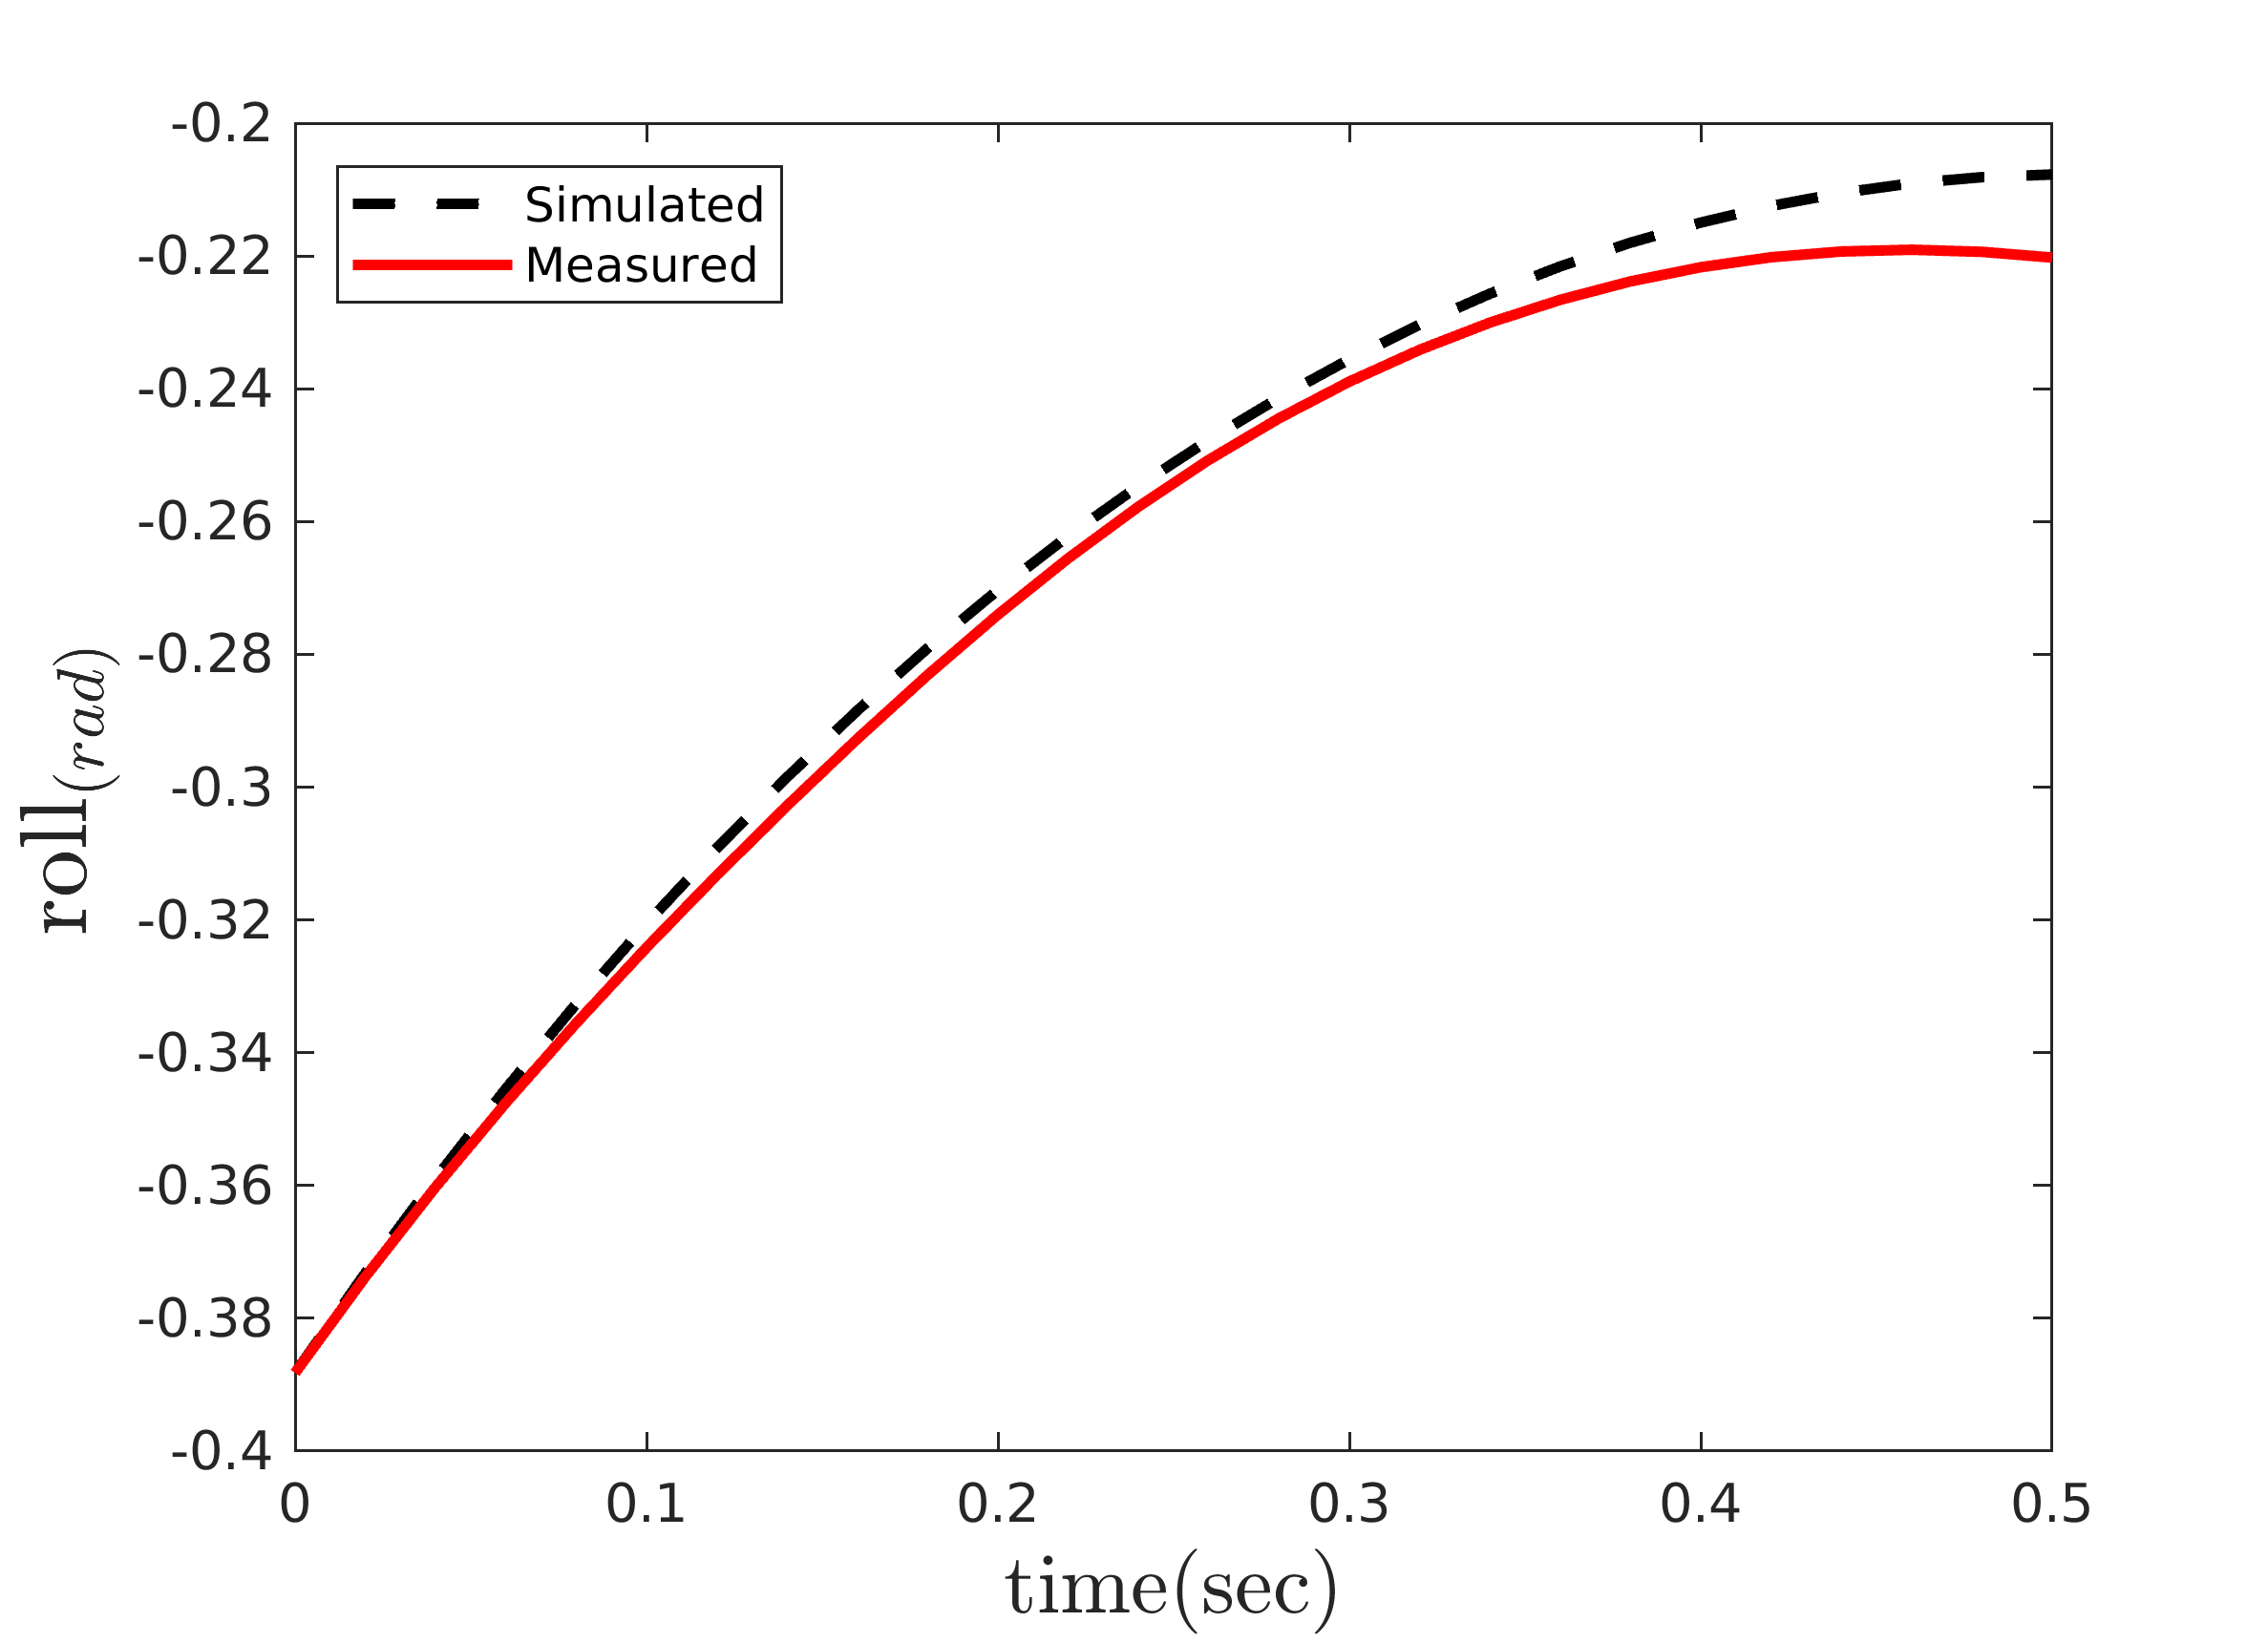
\includegraphics[width=12cm]{../Figures/RCP/roll_ml_parameter_estimation/RCP_roll_S1.png}
%	\centering
%	\caption{مقايسه وضعیت استند در  آزمايش اول و شبیه‌سازی، پس از تخمین پارامترهای کانال رول موتور خاموش}
%	\label{roll_ml_ps1}
%\end{figure}





  \begin{minipage}[H]{\linewidth}
	\hfill
	\begin{minipage}[b]{0.49\linewidth}
		\centering
		\begin{tabular}{ccc}\hline
			 پارامتر & مقدار اولیه  & مقدار بعد از اصلاح
			 \\ \hline
			$A_1$  & $7.312$ & $4.152$ \\
			$A_5$ & $0.0087$ & $0.0190$\\
			$A_6$ & $0.51$ & $0.65$\\ \hline
			\\\\
		\end{tabular}
	\captionsetup{justification=centering}
		\captionof{table}{مقايسه پارامترهای کانال رول موتور خاموش قبل و بعد از اصلاح}
	\end{minipage}
	\begin{minipage}[b]{0.48\linewidth}
		\centering
		\captionsetup{justification=centering}
		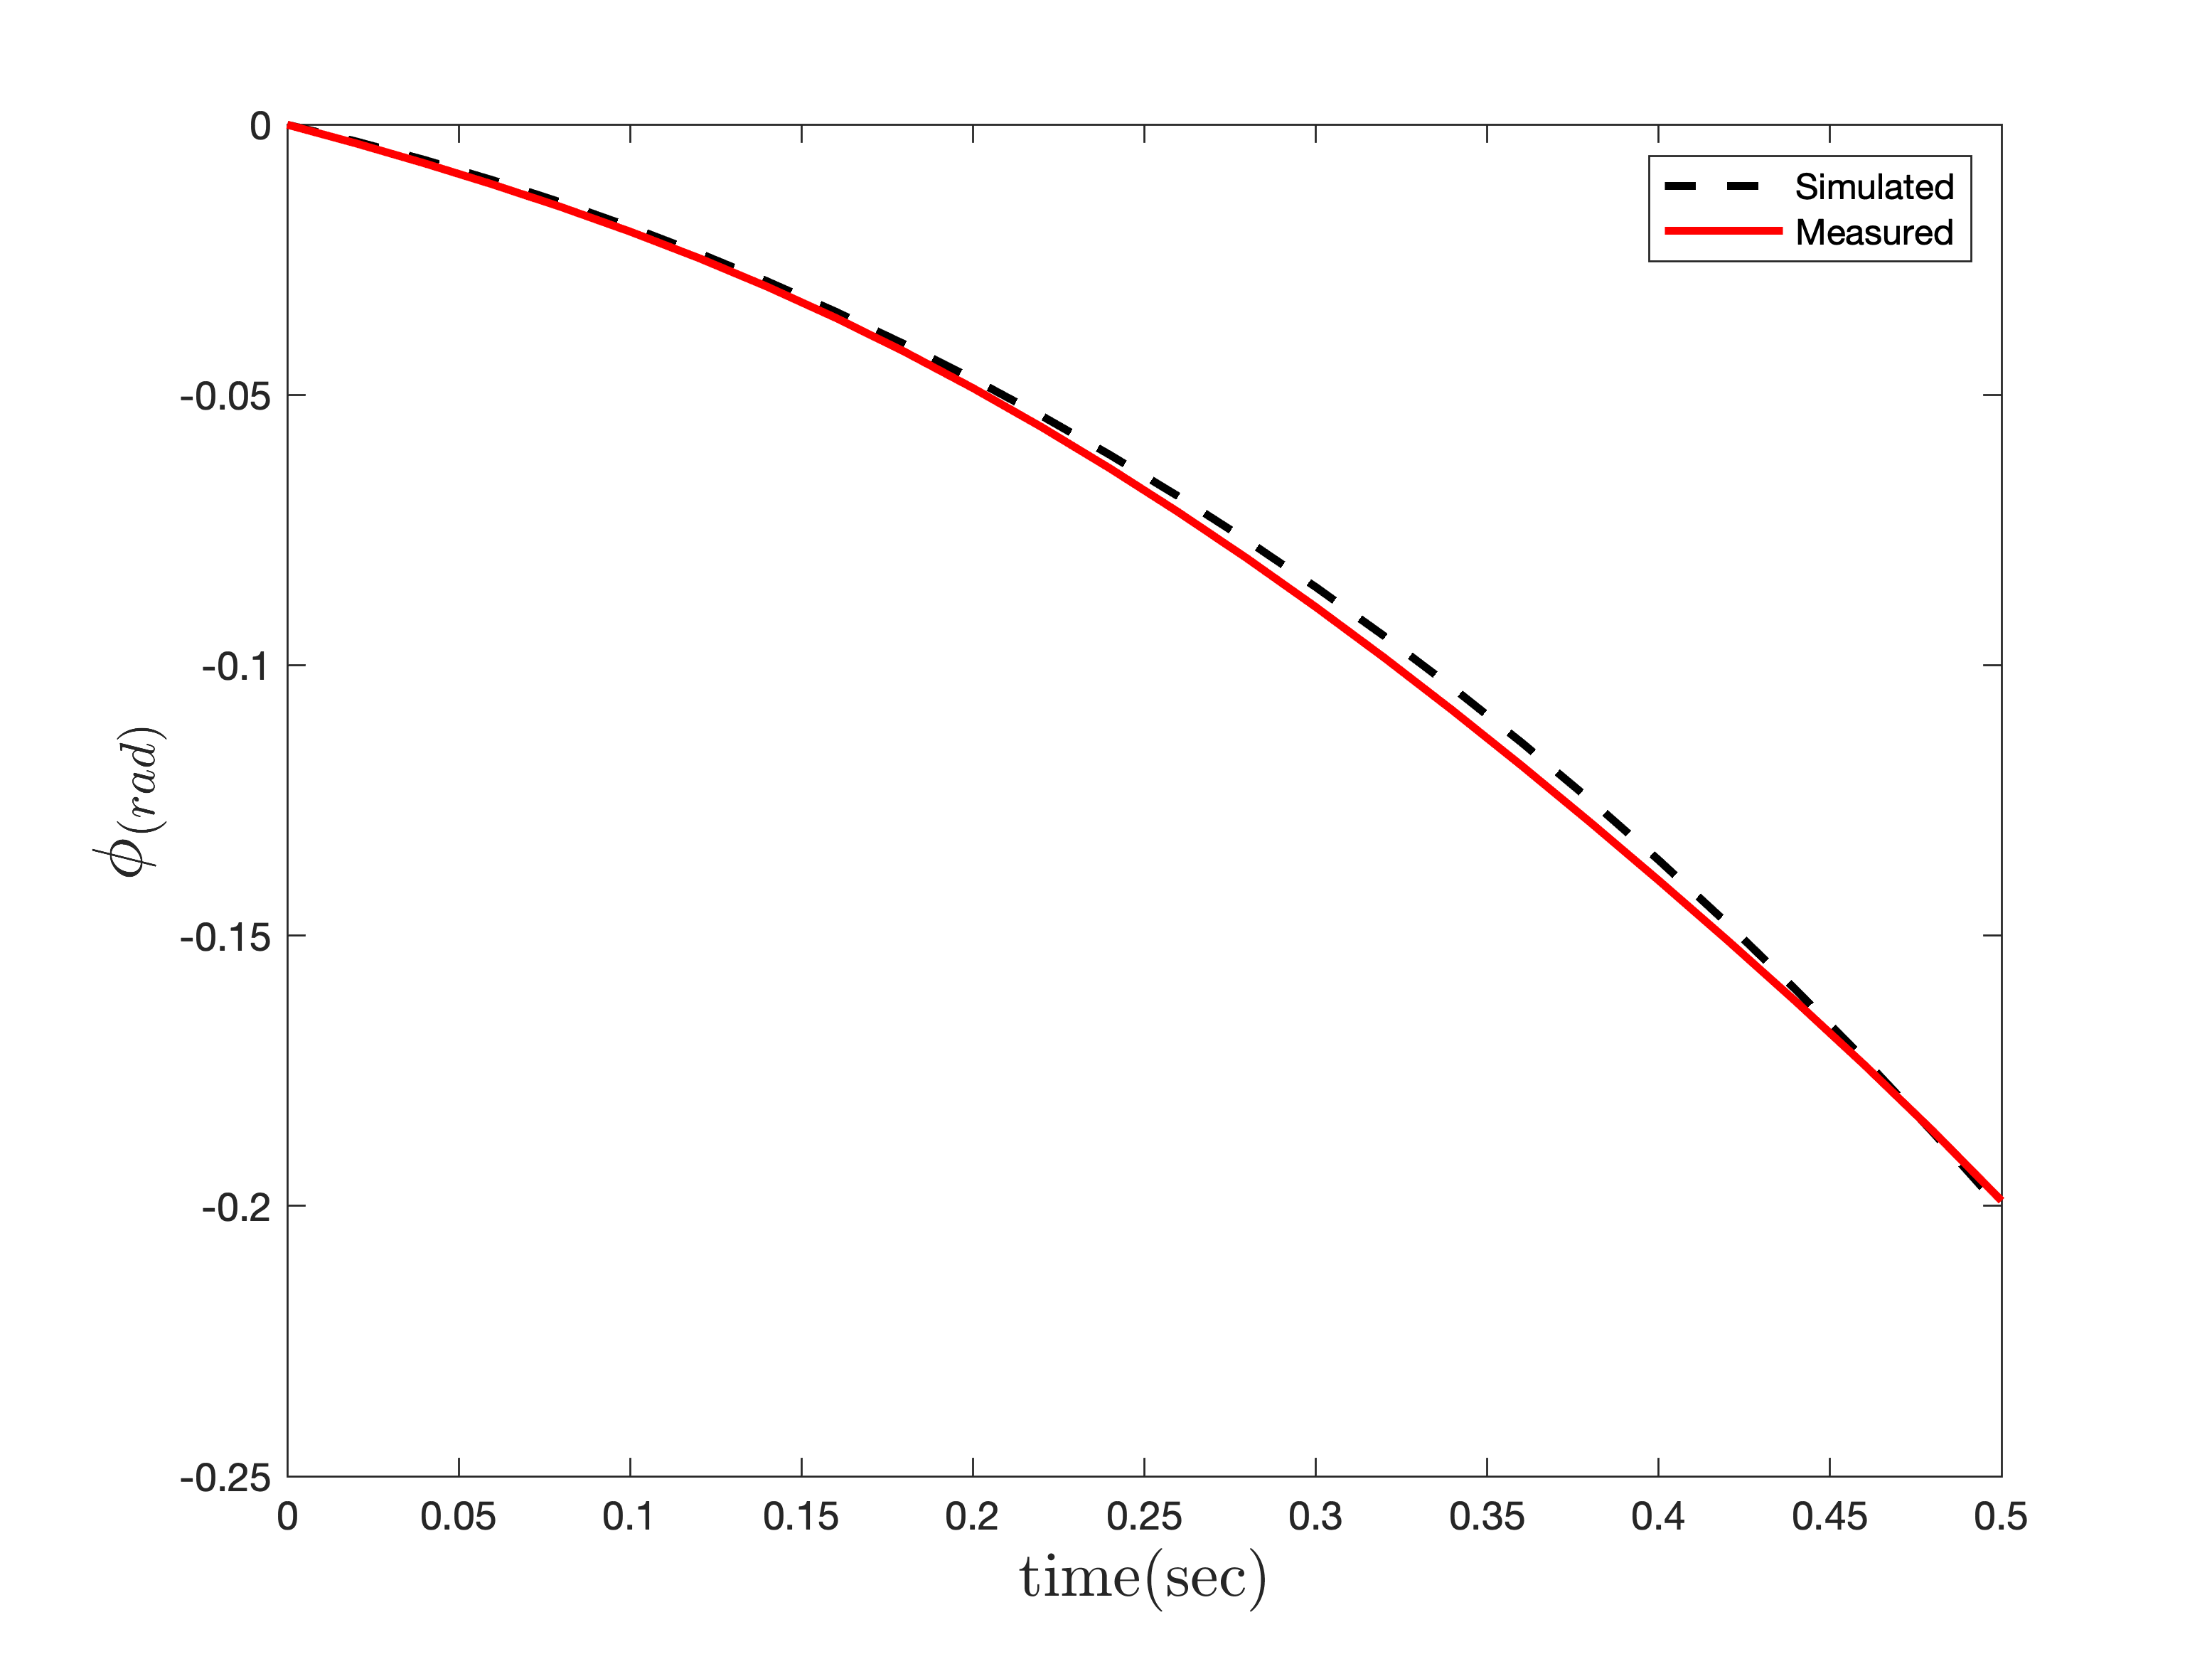
\includegraphics[width=1\linewidth]{../Figures/RCP/roll_ml_parameter_estimation/RCP_roll_S2.png}
		\captionof{figure}{مقايسه وضعیت کانال رول موتور خاموش در شبیه‌سازی و واقعیت}
	\end{minipage}
\end{minipage}

\vspace{0.5cm}
%\begin{figure}[H]
%	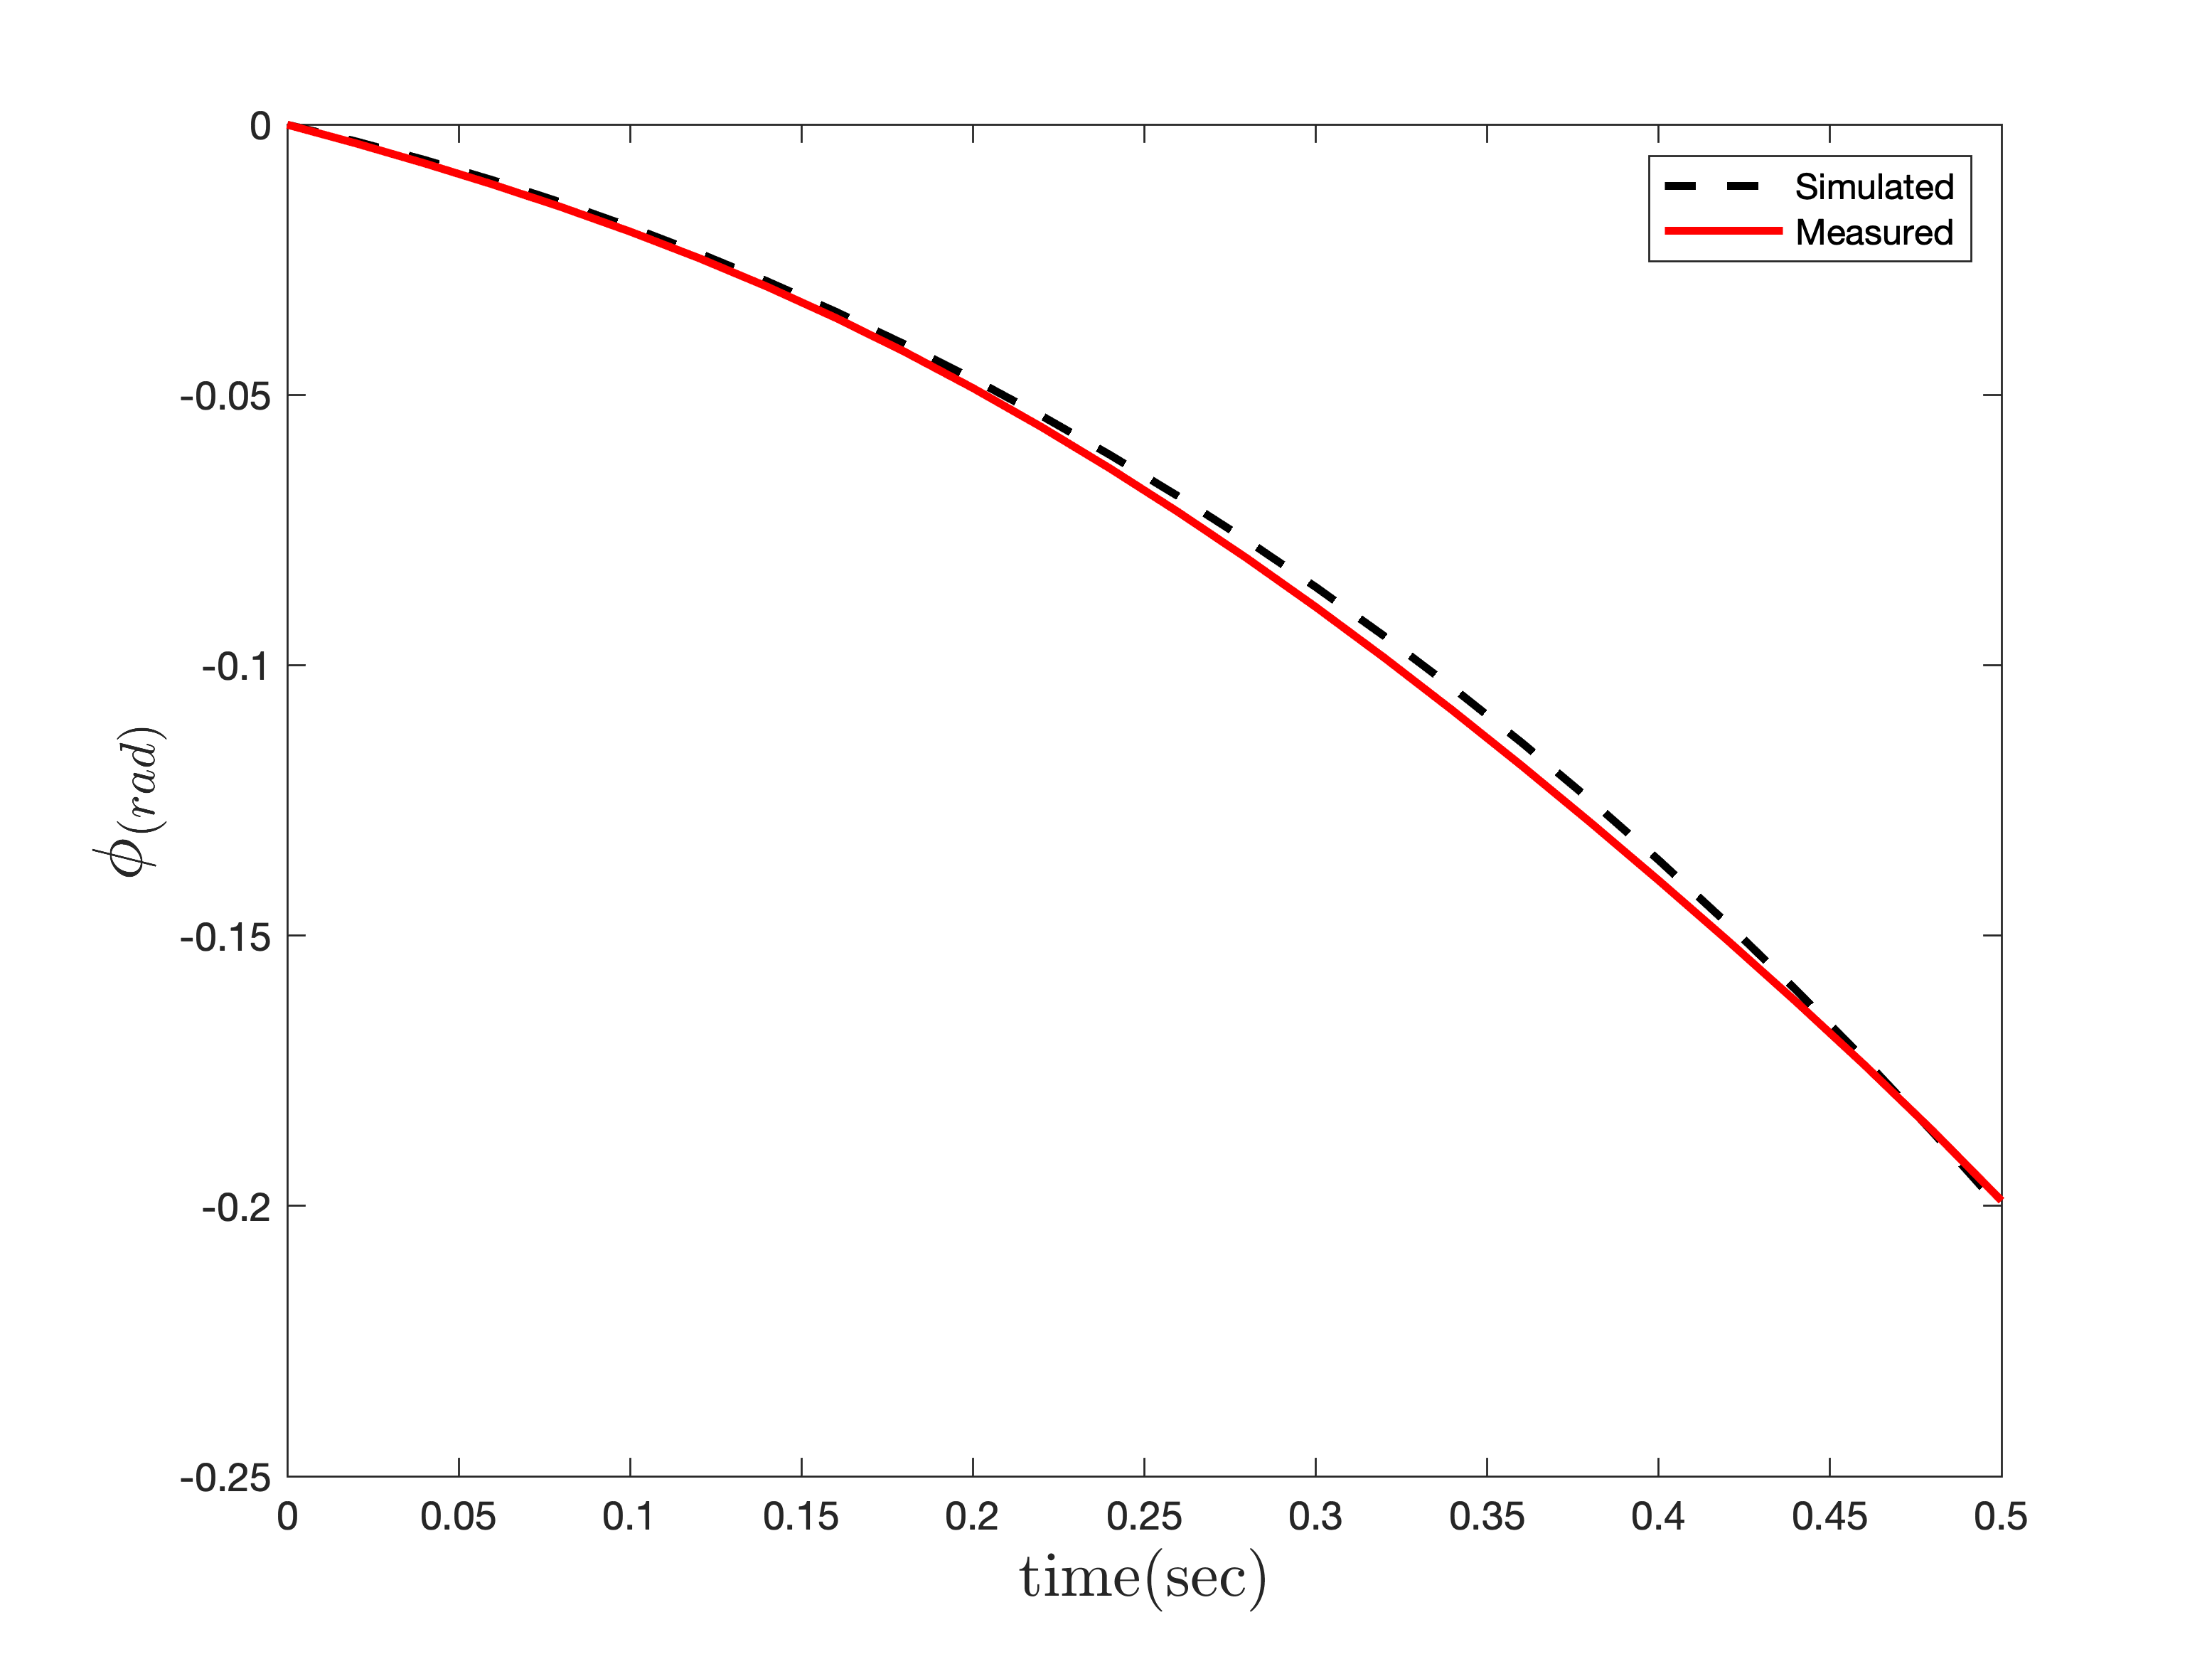
\includegraphics[width=.48\linewidth]{../Figures/RCP/roll_ml_parameter_estimation/RCP_roll_S2.png}
%	\centering
%	\caption{مقايسه وضعیت استند در  آزمايش دوم و شبیه‌سازی، پس از تخمین پارامترهای کانال رول موتور خاموش}
%	\label{roll_ml_ps2}
%\end{figure}
%\begin{figure}[H]
%	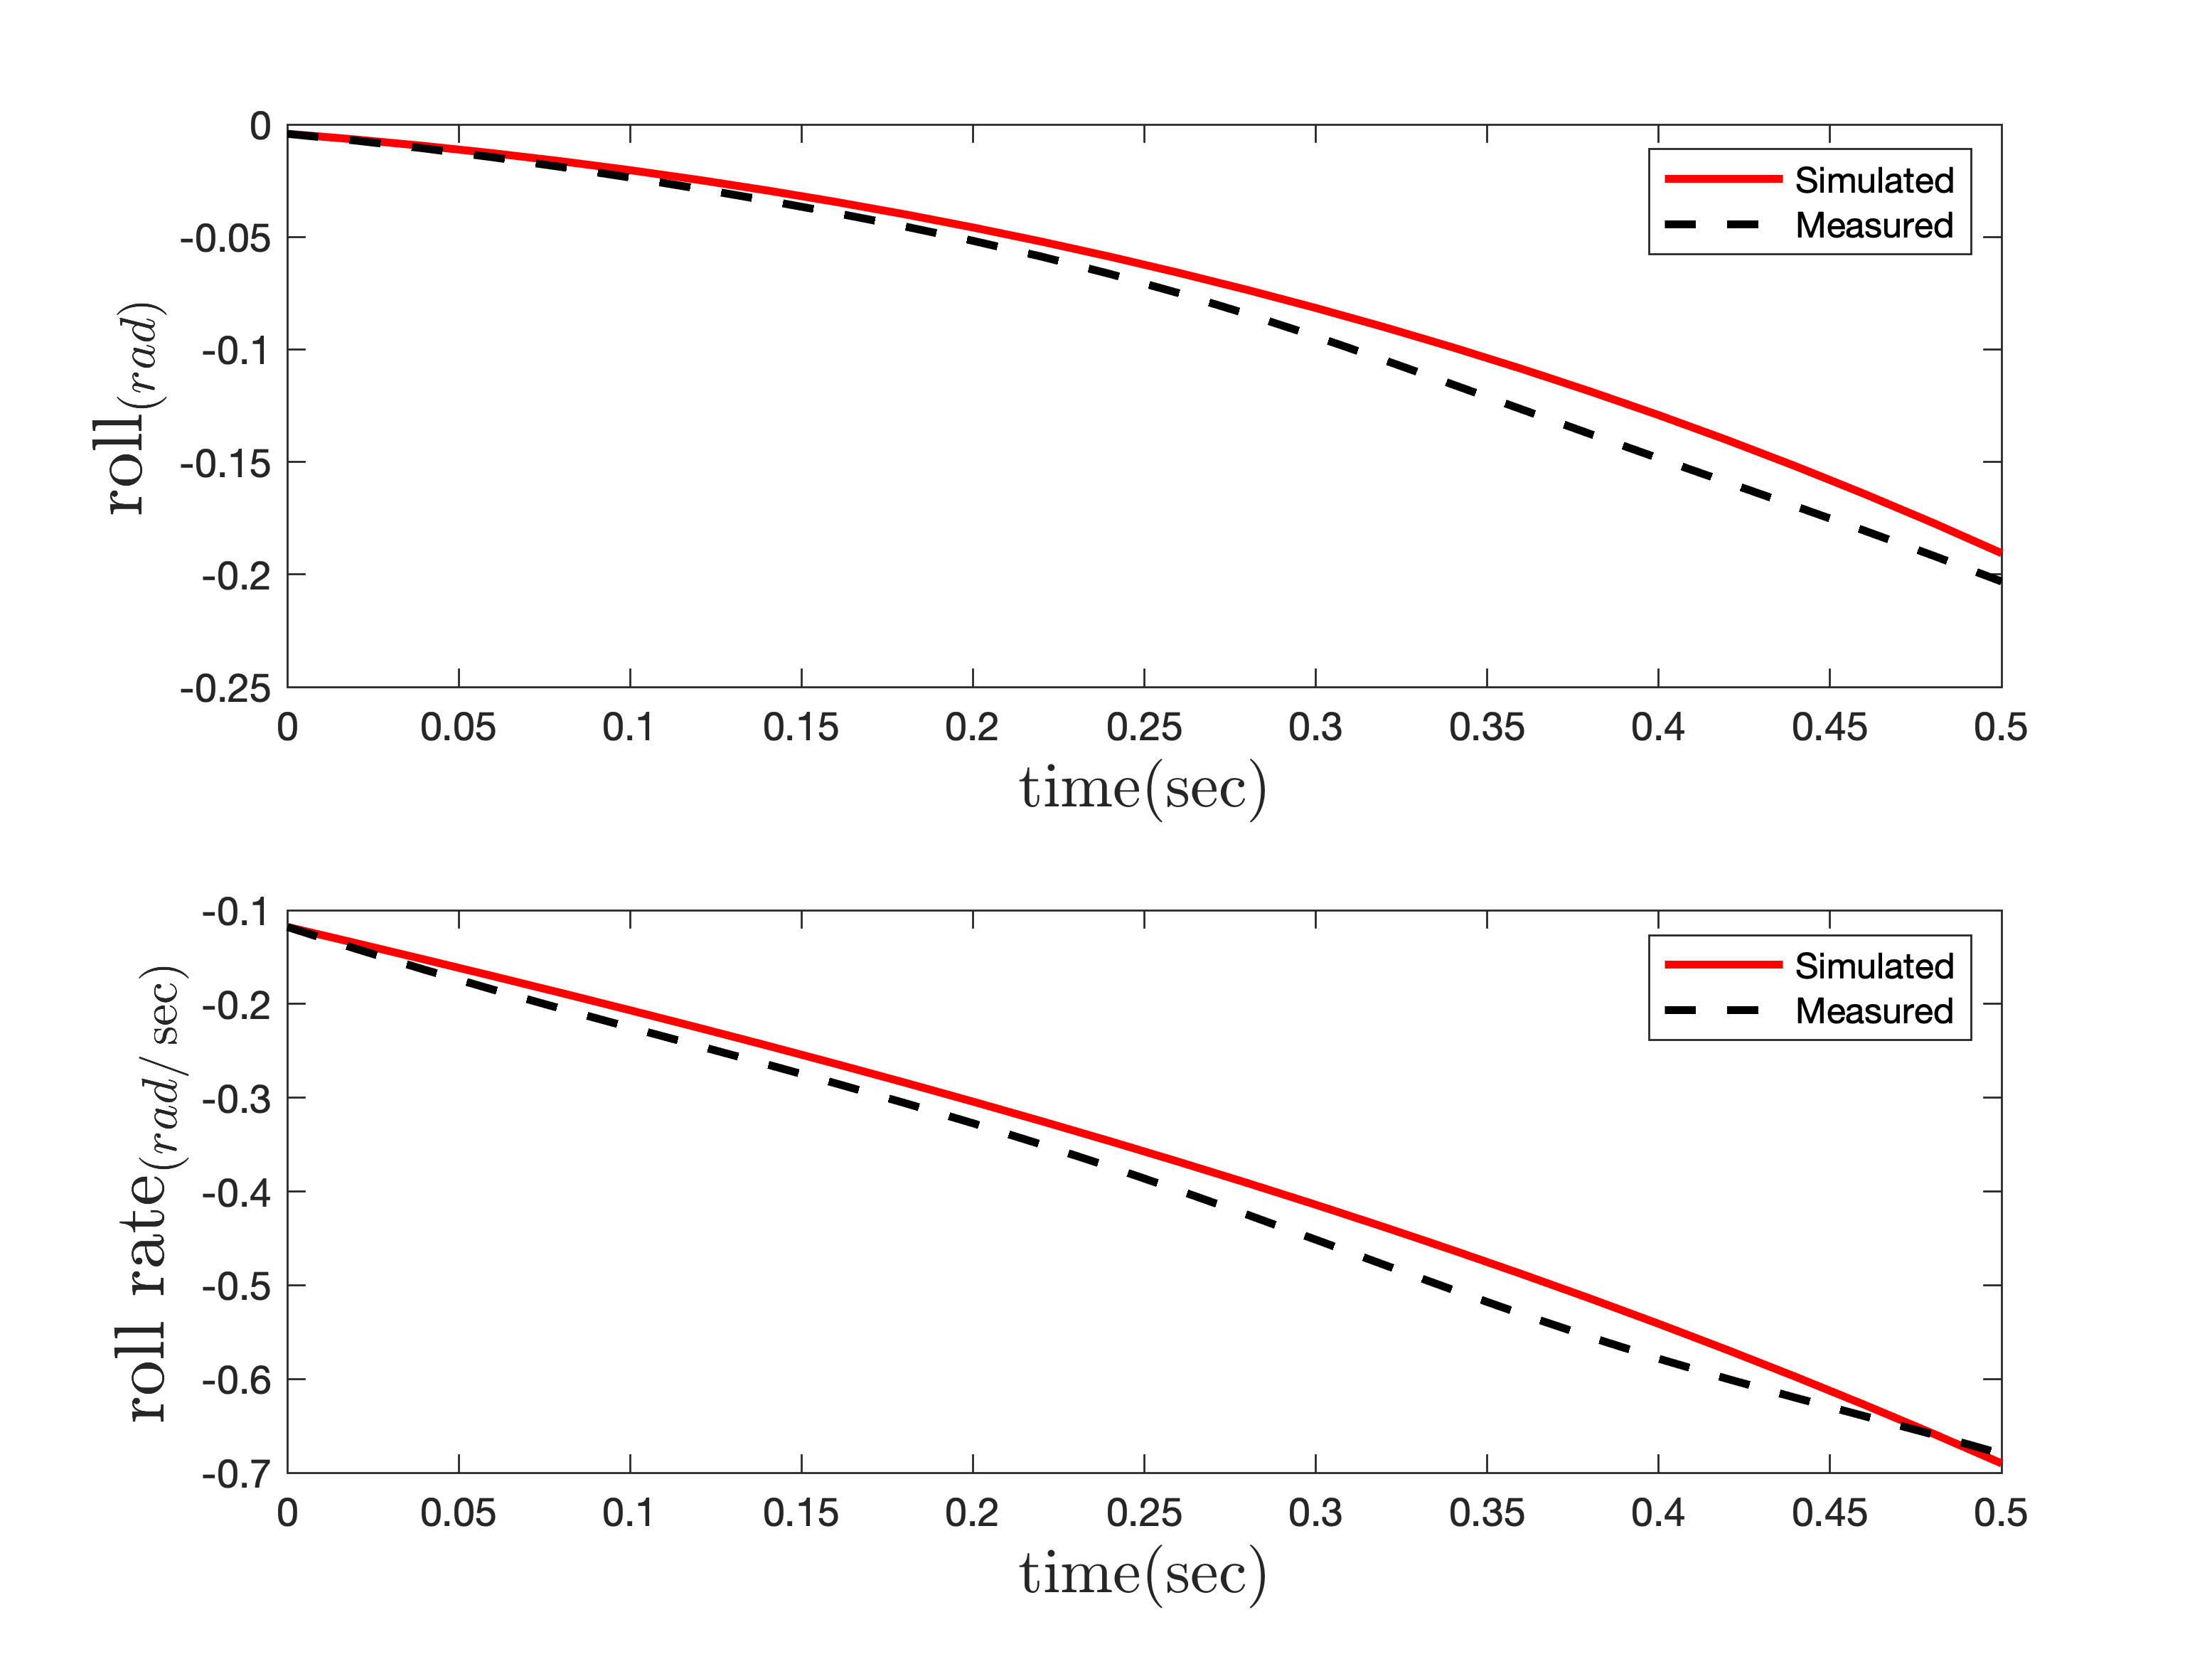
\includegraphics[width=12cm]{../Figures/RCP/roll_ml_parameter_estimation/RCP_roll_S3.png}
%	\centering
%	\caption{مقايسه وضعیت استند در  آزمايش سوم و شبیه‌سازی، پس از تخمین پارامترهای کانال رول موتور خاموش}
%	\label{roll_ml_ps3}
%\end{figure}
%\begin{figure}[H]
%	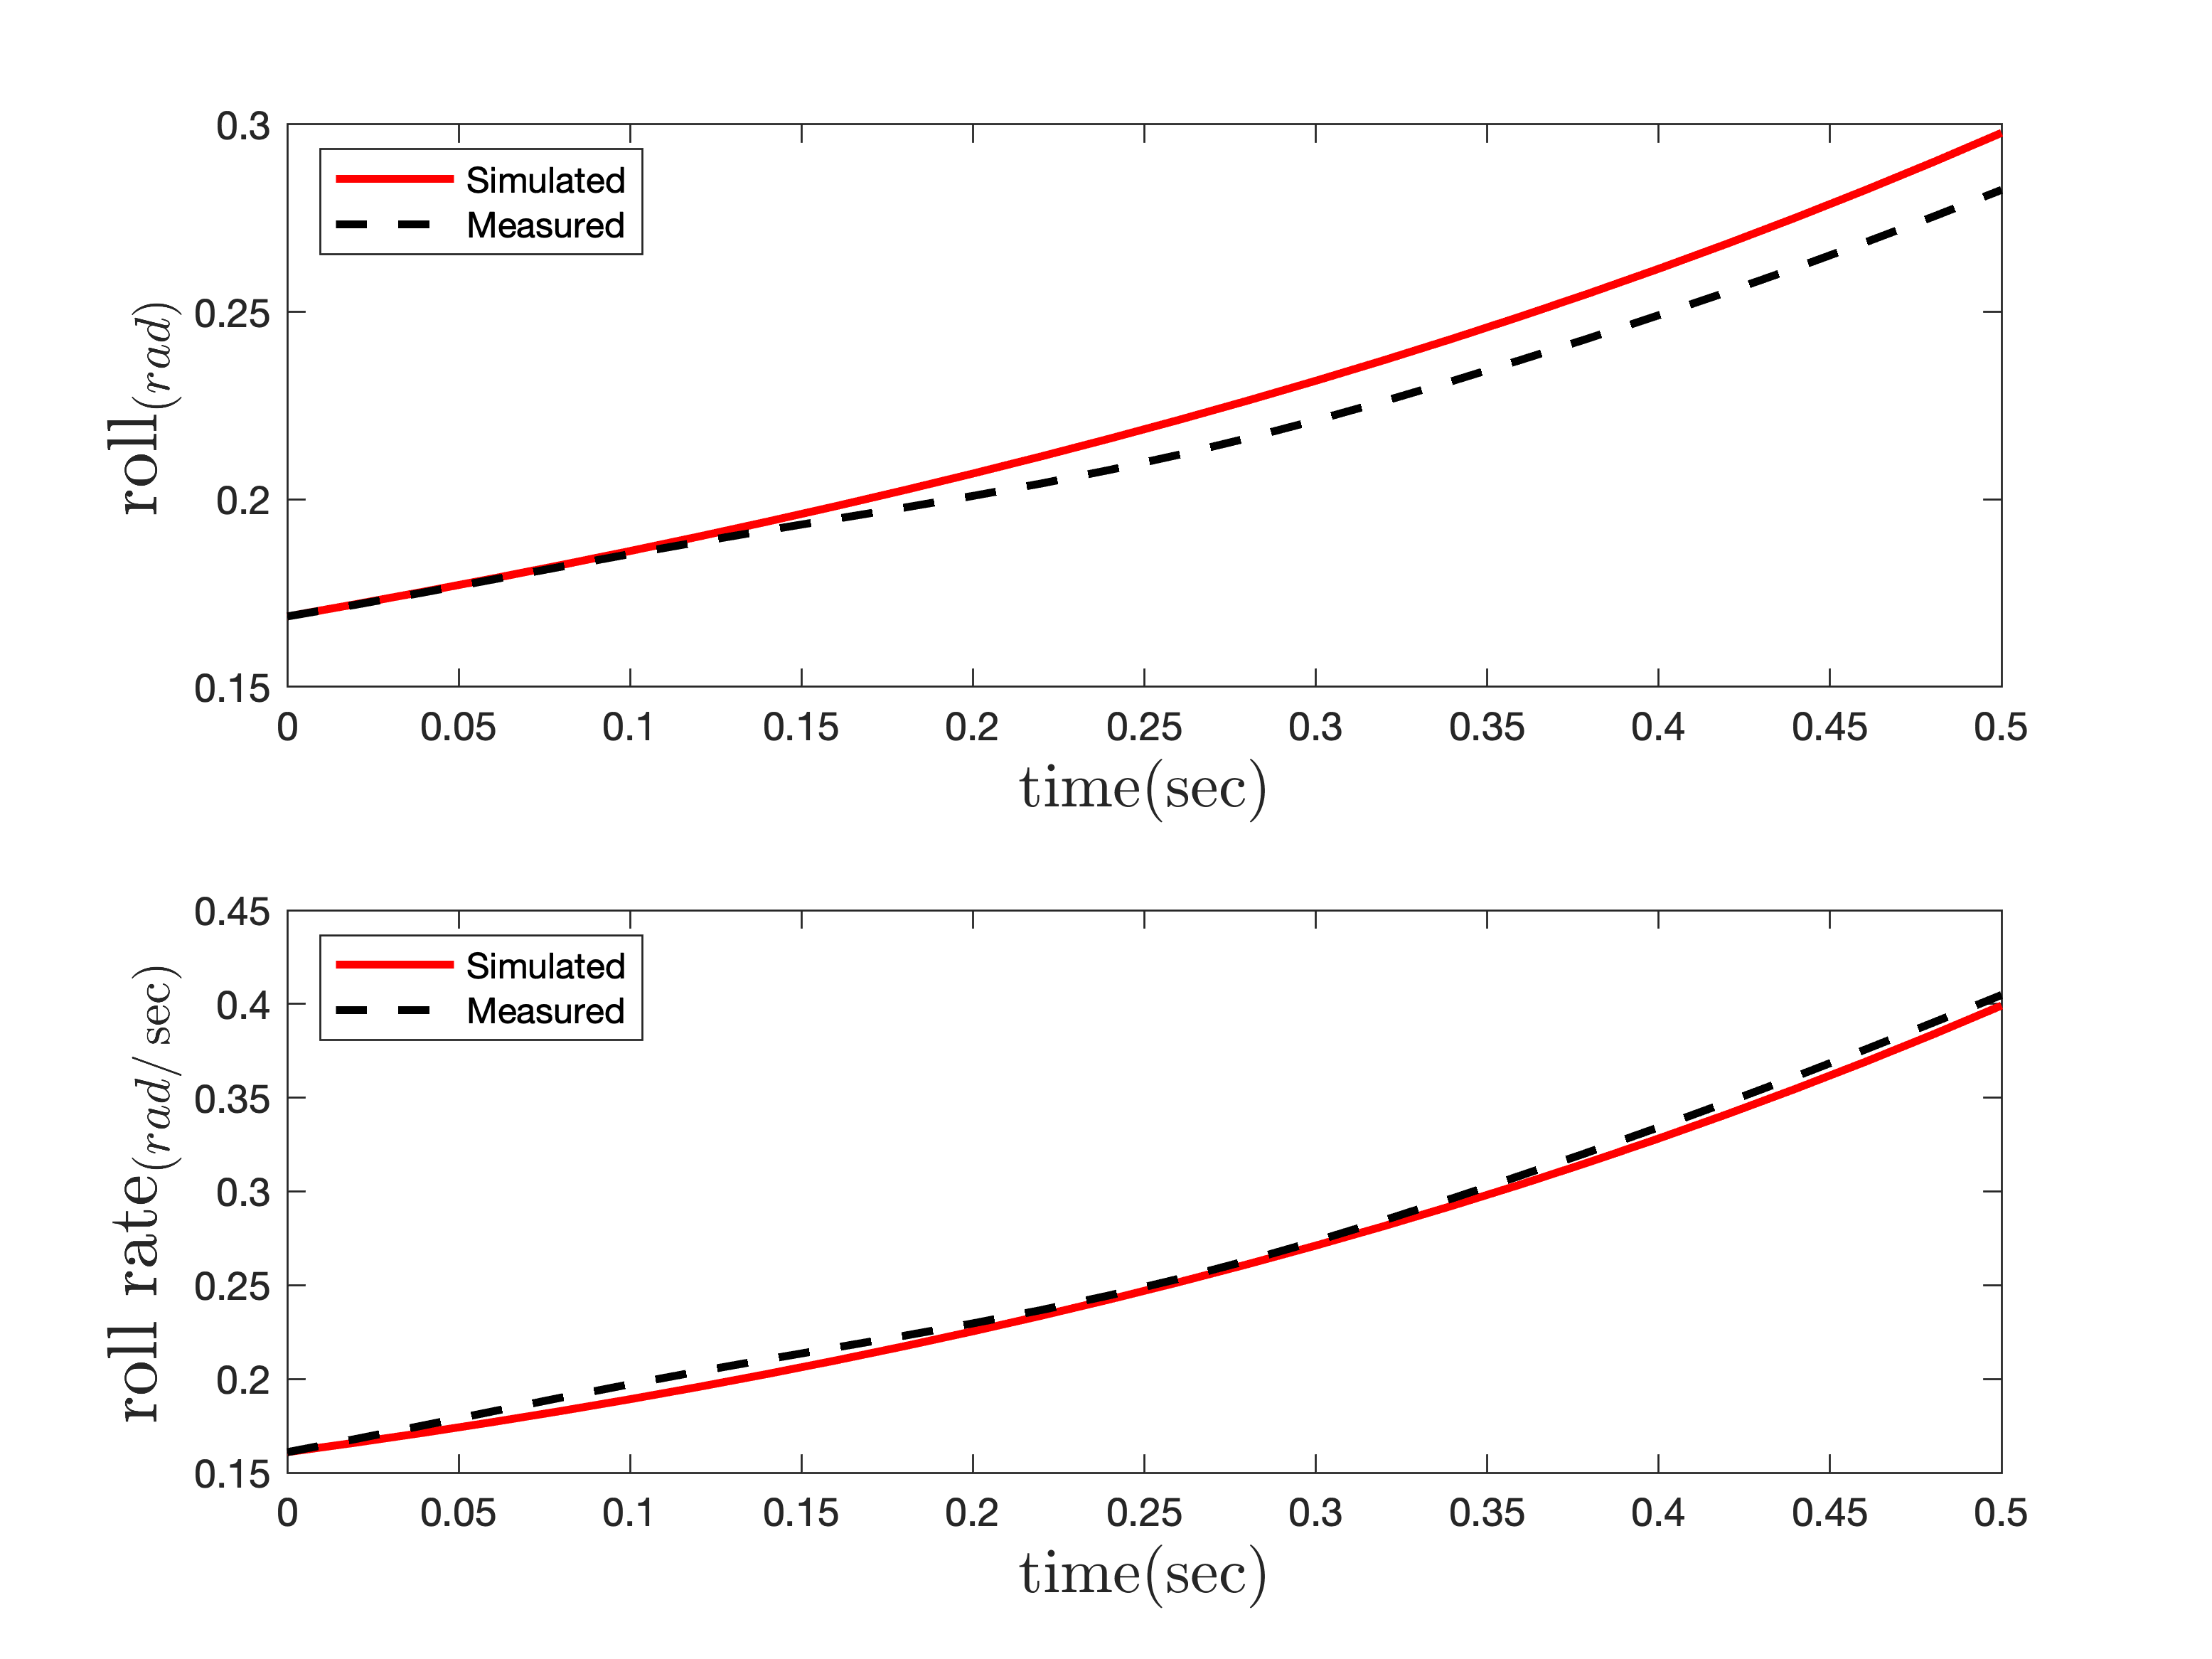
\includegraphics[width=12cm]{../Figures/RCP/roll_ml_parameter_estimation/RCP_roll_S4.png}
%	\centering
%	\caption{مقايسه وضعیت استند در  آزمايش چهارم و شبیه‌سازی، پس از تخمین پارامترهای کانال رول موتور خاموش}
%	\label{roll_ml_ps4}
%\end{figure}
